%==============================================================================
%
% Scientia cum Industria - LaTeX Template V. 1.1
%
%==============================================================================
\documentclass[journal,twoside,a4paper]{SCIndustria}
\usepackage[utf8]{inputenc}
\usepackage{multicol}
\usepackage{amsmath}
\usepackage{graphicx}
\usepackage{epsfig}
\usepackage{caption}
\usepackage{subfigure}
\usepackage[hidelinks]{hyperref}
\usepackage[acronym,nomain]{glossaries}
\usepackage[nameinlink,noabbrev]{cleveref}
\usepackage{siunitx}
\usepackage{float}

\NewDocumentCommand{\xref}{m m}{\hyperref[#1]{#2}}

\NewDocumentCommand{\Eqref}{m}{\Cref{#1}}
\NewDocumentCommand{\eqlabel}{m}{\label{#1}}
% There is an \eqref from amsmath I'm overriding here
\RenewDocumentCommand{\eqref}{m}{\cref{#1}}

\NewDocumentCommand{\figlabel}{m}{\label{#1}}
\NewDocumentCommand{\Figref}{m}{\Cref{#1}}
\NewDocumentCommand{\figref}{m}{\cref{#1}}

\NewDocumentCommand{\tablabel}{m}{\label{#1}}
\NewDocumentCommand{\Tabref}{m}{\Cref{#1}}
\NewDocumentCommand{\tabref}{m}{\cref{#1}}

\newacronym{tecolab}{TeCoLab}{Temperature Control Laboratory}
\newacronym{lti}{LTI}{Linear Time-Invariant}
\newacronym{pid}{PID}{Proportional Integral Derivative}
\newacronym{pd}{PD}{Proportional Derivative}
\newacronym{ff}{FF}{Feed-Forward}
\newacronym{ess}{$E_{ss}$}{Steady-State Error}
\newacronym{zoh}{ZOH}{Zero-Order Hold}
\newacronym{fopdt}{FOPDT}{First Order Plus Dead Time}
\newacronym{rmse}{RMSE}{Root Mean Squared Error}

\newcommand\blfootnote[1]{%
  \begingroup
  \renewcommand\thefootnote{}\footnote{#1}%
  \addtocounter{footnote}{-1}%
  \endgroup
}

\markboth
{Universidade de Caxias do Sul, v. X, n. Y, pp. PP –- PP, 2026} {Universidade de
Caxias do Sul, v. X, n. Y, pp. PP –- PP, 2026}

\begin{document}
\title{Identification of the dynamics of a thermal plant and designing a digital LTI controller for the TeCoLab system}

\author{Gabriel Rodrigues Tavares, Gabriel Tomazzoni Mazzarotto}

\twocolumn[
\begin{@twocolumnfalse}

\maketitle
\blfootnote{}
\blfootnote{Data de envio: 18/06/2026}
\blfootnote{Data de aceite: 18/06/2026}
\vspace{-1cm}
\begin{resumo}
This paper presents the identification and digital control of a thermal plant for the \gls{tecolab} platform. A mathematical model of the plant was obtained from experimental data and used in the design of a digital \gls{lti} controller capable of tracking a specified reference signal. The controller performance was evaluated through simulations and experimental validation and quantified using the \gls{rmse} performance metric.
\end{resumo}
{\small
\begin{center}
{\bfseries Palavras-chave}\\
digital control, Ziegler--Nichols, PID controller, \textit{feed-forward}, TeCoLab, thermal plant
\end{center}
}
\vspace{.5cm}
\end{@twocolumnfalse}
] { \renewcommand{\thefootnote}%
    {\fnsymbol{footnote}}

\glsresetall%
\section{Introduction}
The objective of this paper is to identify the dynamics of a thermal plant from
a physical system known as \gls{tecolab} and to implement a discrete-time
\gls{lti} controller with a sampling period of \SI{15}{\second}. The proposed
controller is designed to track a reference signal with the smallest possible
error, taking zero steady-state error as the ideal performance criterion.

To achieve this objective, plant identification techniques based on sensor
measurements will be employed, including the Ziegler--Nichols step-response
method. In addition, \gls{lti} control strategies, such as \gls{pid} control,
will be used to obtain the best possible tracking performance with respect to
the reference signal.

The proposed methods will be validated through both simulations and experimental
tests conducted on the \gls{tecolab} platform.


\section{Plant modeling and identification}
From a step-response test with an input amplitude of $50^\circ\mathrm{C}$
applied to heater 1, the plant dynamics were identified. The feedback signal is
based on sensor 1, while the tracking objective refers to the relative
temperature measured by sensor 2. The Ziegler-Nichols step-response method was
adopted using a \gls{fopdt} model, yielding an approximation for each sensor, as
given by \Eqref{planta-sensor-1-zn,planta-sensor-2-zn}:

\begin{align}
\eqlabel{planta-sensor-1-zn}
G_{1}(s) &= \frac{0.92}{188.03s + 1} \cdot e^{-6.37s}\\
\eqlabel{planta-sensor-2-zn}
G_{2}(s) &= \frac{0.91}{183.94s + 1} \cdot e^{-11.66s}
\end{align}

The sensor 1 model, which was used for controller design, was discretized using
\gls{zoh} with $T_s = \SI{15}{\second}$, resulting in \Eqref{planta-gz-zoh}.

The model was evaluated by comparing the step response of the \gls{fopdt} model with the experimental data, showing good agreement in both the static gain and the identified time constant.

\section{Controller design}
The controller was designed using a parallel \gls{pd} structure. The initial
gains were obtained using the Ziegler--Nichols tuning method based on
\Eqref{planta-sensor-1-zn} and were subsequently refined using the \gls{rmse},
defined by \Eqref{rmse}, as the performance criterion.

\begin{equation}
\eqlabel{rmse}
\mathrm{RMSE} = \sqrt{\frac{1}{N}\sum_{k=1}^{N}{\left( r[k] - y[k] \right)}^{2}}
\end{equation}

The resulting \gls{pd} controller is given by \Eqref{controlador-pd-paralelo}.

\begin{equation}
\eqlabel{controlador-pd-paralelo}
C_{\mathrm{pd}}(s) = 13.472 + \frac{601.4s}{s+100}
\end{equation}

Although the \gls{pd} controller provided satisfactory dynamic performance, it
still exhibited a noticeable \gls{ess} when tracking the reference signal.

To reduce this error, a \gls{ff} action was added based on an inverse plant
model combined with a filter that specifies the desired closed-loop
dynamics~\cite{astrom2021feedback,seborg2016process}.
This control strategy uses the process model to anticipate the control action
required for reference tracking~\cite{astrom2021feedback}.

In this paper, the \gls{ff} controller was implemented using the inverse model
of the plant described by \Eqref{planta-sensor-1-zn}, operating in parallel with
the \gls{pd} controller, together with a low-pass filter to ensure causality.
The resulting feed-forward controller is given by \Eqref{controlador-ff}:

\begin{equation}
\eqlabel{controlador-ff}
C_{\mathrm{ff}} = \frac{188.0271s + 1}{6.075 s + 0.92}
\end{equation}

\Figref{bloco-controlador} shows the complete control structure. The \gls{ff}
controller acts directly on the reference signal, while the \gls{pd} controller
compensates for the tracking error through system feedback.

\begin{figure}[H]
\centering
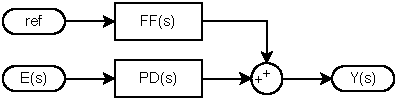
\includegraphics[width=0.9\linewidth]{images/Bloco Controlador.pdf}
\caption{Proposed control structure composed of a \gls{ff} action applied to the
reference signal and a \gls{pd} action based on system feedback.}
\figlabel{bloco-controlador}
\end{figure}

The controller was discretized using the Tustin method, applied to both the
\gls{pd} and \gls{ff} controllers. In this method, the continuous-time operator
$s$ is approximated by the bilinear transformation given in \Eqref{tustin}:

\begin{equation}
\eqlabel{tustin}
s \approx \frac{2}{T_s}\frac{z-1}{z+1}
\end{equation}

Where $T_s$ is the sampling period, defined as $T_s = \SI{15}{\second}$. The
plant model was discretized using \gls{zoh}, resulting in \Eqref{planta-gz-zoh}.

\begin{equation}
\eqlabel{planta-gz-zoh}
G(z) = z^{-1} \cdot \frac{0.0413z + 0.0293}{z - 0.9233}
\end{equation}


\section{Simulation results}
The simulations were made in the Simulink environment using the plant model
identified in \Eqref{planta-sensor-1-zn} and the controllers presented in
\Eqref{controlador-pd-paralelo,controlador-ff}. To approximate the experimental
conditions a white noise was added to the plant output, and a saturation block
was included to represent the maximum heater power.

The results demonstrate that the control strategy combining the \gls{pd} and
\gls{ff} controllers was able to track the reference signal with low tracking
error during both the transient and steady-state regimes.


\section{Experimental results}
The designed controller was implemented in the Python programming language and
deployed on the \gls{tecolab} platform. The system was subjected to the same
reference signal used in the simulations. The experimental results exhibited
behavior consistent with that predicted by the simulations, maintaining a low
tracking error throughout the experiment.


\section{Comparison between simulation and experimental results}
\Figref{grafico-resultados} compares the simulation and experimental results
obtained for the same reference signal. Using the \gls{rmse} metric from
\Eqref{rmse} to evaluate the tracking error of the relative temperature
measured by sensor 2.

The simulated system achieved an $\mathrm{RMSE} = 1.3567,^\circ\mathrm{C}$,
while the experimental test resulted in an
$\mathrm{RMSE} = 2.2956,^\circ\mathrm{C}$. In both cases, the combined \gls{pd}
and \gls{ff} control strategy was able to track the reference signal during both
the ramp transient and steady-state regimes at $40\,^\circ\mathrm{C}$,
recovering from the disturbance introduced at the 10-minute mark.

The approximately $0.94,^\circ\mathrm{C}$ increase in the experimental
\gls{rmse} compared with the simulated result indicates good agreement between
the model and the physical system, although the experimental performance was
slightly worse than that predicted by simulation.

\begin{figure}[H]
\centering
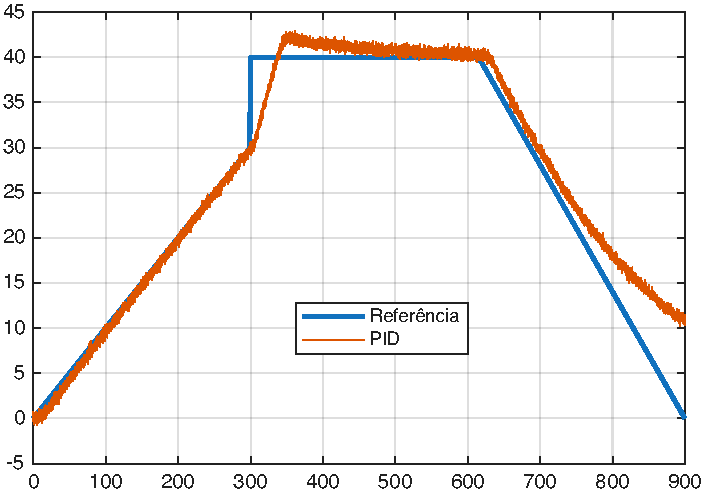
\includegraphics[width=0.9\linewidth]{images/Resultados.pdf}
\caption{Comparison between the simulated and experimental results for tracking
the relative temperature reference measured by sensor 2.}
\figlabel{grafico-resultados}
\end{figure}


\section{Analysis of the observed discrepancies}
The difference between the simulated and experimental \gls{rmse} values
can be attributed to factors not considered in the \gls{fopdt} model used for
the controller design. The main sources of discrepancy include sensor
measurement noise, transport delays, and unmodeled thermal dynamics of the
physical plant.

Another source of discrepancy arises from the system architecture itself, in
which the controller uses the measurement from Sensor 1 for feedback, while the
error is computed based on the temperature measured by Sensor 2. The spatial
separation between the sensors introduces a delay between the controlled
variable and the variable of interest, which was not fully captured by the model
employed in the design process.

The disturbance introduced at 10 minutes, resulting from the activation of a
fan, also contributed to the increase in the experimental error, since its
actual effect on the plant differs from the simplified representation adopted in
the simulation.

Despite these discrepancies, the close agreement between the simulated and
experimental \gls{rmse} values confirms that the identified model adequately
represents the plant dynamics and that the proposed control strategy maintains
good reference-tracking performance under experimental conditions as well.


\section{References}
\bibliographystyle{IEEEbib}
\bibliography{my_refs}

\end{document}